\documentclass{book}

\usepackage{geometry}
\usepackage[utf8]{inputenc}
\usepackage{amsmath}
\usepackage{amsfonts}
\usepackage{amssymb}
\usepackage{graphicx}
\usepackage[utf8]{inputenc}
\usepackage{amsmath}
\usepackage{amsfonts}
\usepackage{amssymb}
\usepackage{listings}
\usepackage{xcolor}
\usepackage[most]{tcolorbox}
\usepackage{mathtools}
\usepackage{float}
\usepackage[colorlinks=false, linktocpage=true]{hyperref}

\usepackage{booktabs}% http://ctan.org/pkg/booktabs
\newcommand{\tabitem}{~~\llap{\textbullet}~~}
\usepackage{longtable}
 
\usepackage{caption}
\DeclareCaptionType{code}[Code Listing][List of Code Listings] 

\definecolor{codegreen}{rgb}{0,0.6,0}
\definecolor{codegray}{rgb}{0.5,0.5,0.5}
\definecolor{codepurple}{rgb}{0.58,0,0.82}
\definecolor{backcolour}{rgb}{0.95,0.95,0.92}
 
\lstdefinestyle{mystyle}{
    backgroundcolor=\color{backcolour},   
    commentstyle=\color{codegreen},
    keywordstyle=\color{magenta},
    numberstyle=\tiny\color{codegray},
    stringstyle=\color{codepurple},
    basicstyle=\ttfamily\footnotesize,
    breakatwhitespace=false,         
    breaklines=true,                 
    captionpos=b,                    
    keepspaces=true,                 
    numbers=left,                    
    numbersep=5pt,                  
    showspaces=false,                
    showstringspaces=false,
    showtabs=false,                  
    tabsize=2
}
 
\lstset{style=mystyle}

\setlength{\parindent}{0em}
\setlength{\parskip}{1em}

\author{Brian Rashap, Ph.D.}
\title{PHYS 1320 - Calculus-based Physics II}

\geometry{letterpaper, portrait, margin=0.75in}

\begin{document}
\frontmatter

\maketitle


\mainmatter

\chapter{Module 1: Chapter 5 - Electric Charges and Fields}

From Newton's Second Laws of Mechanics:

\begin{equation}
F = ma
\end{equation}

A force can be recognized by the effect it has on an object. When studying gravitation, we examined the force of gravity that acts on all objects with mass. Similarly, the electric force acts on all objects with a property called charge. While gravity is an attractive force, the electric force can be either attractive or repulsive.  

\section{Section 5.1 Electric Charge}

The ancient Greek philosopher Thales of Miletus (624-546 BCE)recorded that when amber was vigorously rubbed with a piece of fur, it created a force that attracted them to each other. They also attracted other non-metallic objects even when not touched. 

\begin{figure}[h]
\begin{center}
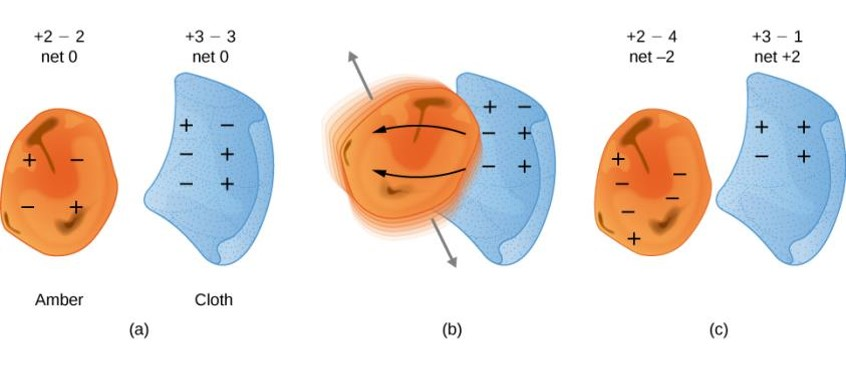
\includegraphics[scale=0.40]{fig/fig_05_05.jpg}
\caption{Materials rubbed together}
\label{fig:05_05}
\end{center}
\end{figure}

The English physicist William Gilbert (1544-1603) also studied attractive forces. He worked with a variety of substances. His findings included:
\begin{itemize}
\item Metals never exhibited this force, whereas minerals did
\item Two "electrified" amber rods would repel each other. 
\end{itemize}

This suggested that were two types of electric properties: attractive and repulsive. This property came to be known as Electric Charge. The force is repulsive between between the same type of charge and attractive between the charges are of opposite types. Named after French physicist Charles Augustine de Coulomb (1736-1806), the unit of electric charge is the coulomb (C).

The American statesman and scientist Benjamin Franklin found that he could concentrate charge in Leyden jar \footnote{Its invention was a discovery made independently by German cleric Ewald Georg von Kleist on 11 October 1745 and by Dutch scientist Pieter van Musschenbroek of Leiden (Leyden), Netherlands in 1745–1746. The invention was named after the city.} (a glass jar with two metal sheets one on the inside and one on the outside (essentially what we now call a capacitor). Franklin pointed out that the behavior could be explained by one type of charge remaining motionless and the other charge flowing from one piece of foil to the other. He had no way of determining which type of charge was moving, and unfortunately he guessed wrong: it was since learned that the charges that flow are the ones that Franklin named "negative" and the "positive" charges remain motionless.

\begin{figure}[h]
\begin{center}
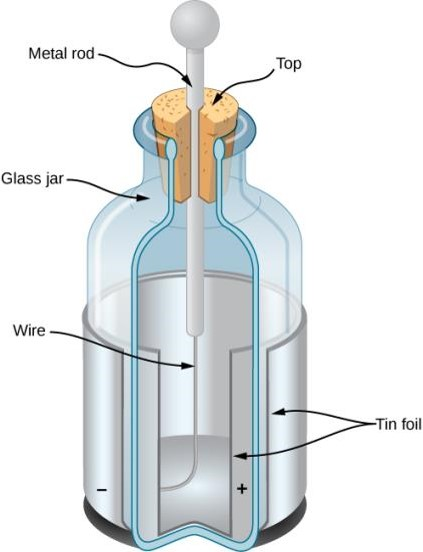
\includegraphics[scale=0.40]{fig/fig_05_06.jpg}
\caption{Leyden Jar}
\label{fig:05_06}
\end{center}
\end{figure}

Observations about the Electric Force:
\begin{itemize}
\item The force acts without physical contact between objects
\item The force is attractive or repulsive
\item Not all objects are affected by this force
\item The magnitude of the force decreases rapidly with distance between objects
\end{itemize}

Properties of Electric Charge
\begin{itemize}
\item Charge is quantized - The smallest amount of charge an object can have is $e = 1.602 * 10^{-19} C$. The charge on any object must be an integer multiple of $e$.
\item The magnitude of a change is independent of the type. The smallest positive charge is $1.602 * 10^{-19} C$ and the smallest negative charge is $-1.602 * 10^{-19} C$; these values are exactly equal in magnitude. 
\item Charge is conserved. Change can not be created or destroyed. It can only be transferred. The net charge of the universe is constant. 
\item Charge is conserved in a closed system. Total charge in a closed system remains constant.
\end{itemize}
These last two items are referred to as the Law of Conservation of Charge. 

\subsection{The Sources of Charge: The Structure of the Atom}

Atomic structure terminology
\begin{itemize}
\item Electron
\item Proton
\item Neutron
\item Ion
\end{itemize}

This simplified model of a hydrogen atom shows a positively charged nucleus (consisting, in the case of hydrogen, of a single proton), surrounded by an electron “cloud.” The charge of the electron cloud is equal (and opposite in sign) to the charge of the nucleus, but the electron does not have a definite location in space;  hence, its representation here is as a cloud. Normal macroscopic amounts of matter contain immense numbers of atoms and molecules, and, hence, even greater numbers of individual negative and positive charges. 

\begin{figure}[h]
\begin{center}
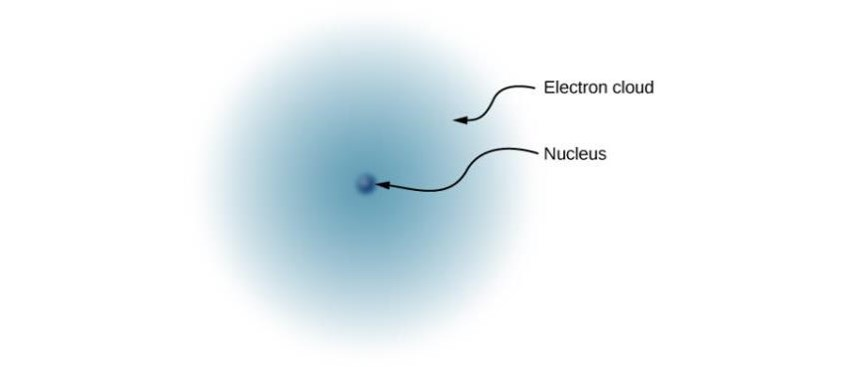
\includegraphics[scale=0.40]{fig/fig_05_07.jpg}
\caption{Simplified model of a hydrogen atom}
\label{fig:05_07}
\end{center}
\end{figure}

The nucleus of a carbon atom is composed of six protons and six neutrons. As in hydrogen, the surrounding six electrons do not have definite locations and so can be considered to be a sort of cloud surrounding the nucleus.


\begin{figure}[h]
\begin{center}
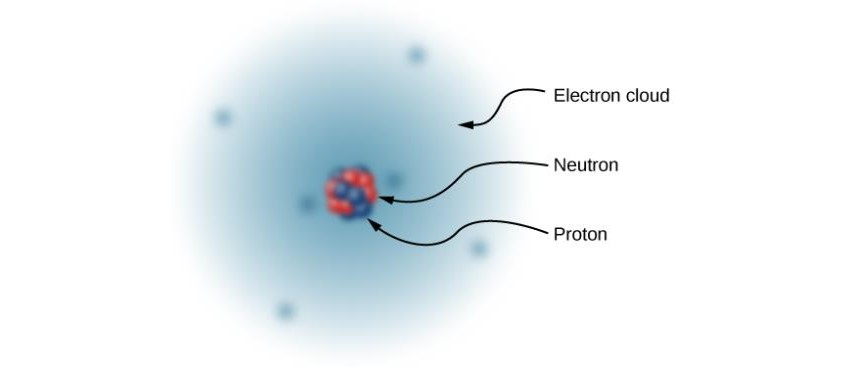
\includegraphics[scale=0.40]{fig/fig_05_08.jpg}
\caption{Carbon atom}
\label{fig:05_08}
\end{center}
\end{figure}

\section{Conductors, Insulators, and Charging by Induction}

\subsection{Conductors}

Electrons surround the tiny nucleus in the form of a (comparatively) vast cloud of negative charge. However, this cloud does have a definite structure to it. If we consider an atom of copper, there is an outermost electron that is only loosely bound to the atom’s nucleus. It can be easily dislodged; it then moves to a neighboring atom. In a large mass of copper atoms (such as a copper wire or a sheet of copper), these vast numbers of outermost electrons (one per atom) wander from atom to atom, and are the electrons that do the moving when electricity flows. These wandering, or “free,” electrons are called conduction electrons, and copper is therefore an excellent conductor (of electric charge). All conducting elements have a similar arrangement of their electrons, with one or two conduction electrons. This includes most metals.

\subsection{Insulators}

Insulators, in contrast, are made from materials that lack conduction electrons; charge flows only with great difficulty, if at all. Even if excess charge is added to an insulating material, it cannot move, remaining indefinitely in place. This is why insulating materials exhibit the electrical attraction and repulsion forces described earlier, whereas conductors do not; any excess charge placed on a conductor would instantly flow away (due to mutual repulsion from existing charges), leaving no excess charge around to create forces. Charge cannot flow along or through an insulator, so its electric forces remain for long periods of time. (Charge will dissipate from an insulator, given enough time.) As it happens, amber, fur, and most semi-precious gems are insulators, as are materials like wood, glass, and plastic.

\subsection{Charging by Induction}

Induced polarization: A positively charged glass rod is brought near the left side of the conducting sphere, attracting negative charge and leaving the other side of the sphere positively charged. Although the sphere is overall still electrically neutral, it now has a charge distribution, so it can exert an electric force on other nearby charges. Furthermore, the distribution is such that it will be attracted to the glass rod.


\begin{figure}[h]
\begin{center}
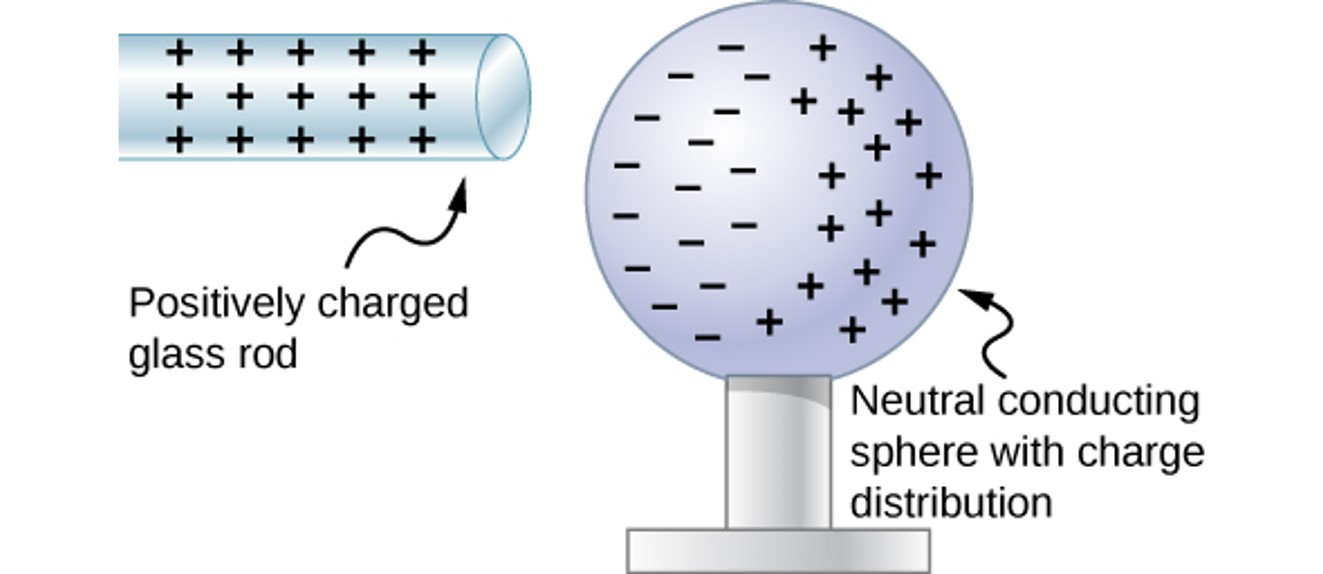
\includegraphics[scale=0.40]{fig/fig_05_10.jpg}
\caption{Induced Polarization}
\label{fig:05_10}
\end{center}
\end{figure}

Both positive and negative objects attract a neutral object by polarizing its molecules.
\begin{itemize}
\item A positive object brought near a neutral insulator polarizes its molecules. There is a slight shift in the distribution of the electrons orbiting the molecule, with unlike charges being brought nearer and like charges moved away. Since the electrostatic force decreases with distance, there is a net attraction.
\item  A negative object produces the opposite polarization, but again attracts the neutral object. 
\item The same effect occurs for a conductor; since the unlike charges are closer, there is a net attraction.
\end{itemize}

\begin{figure}[h]
\begin{center}
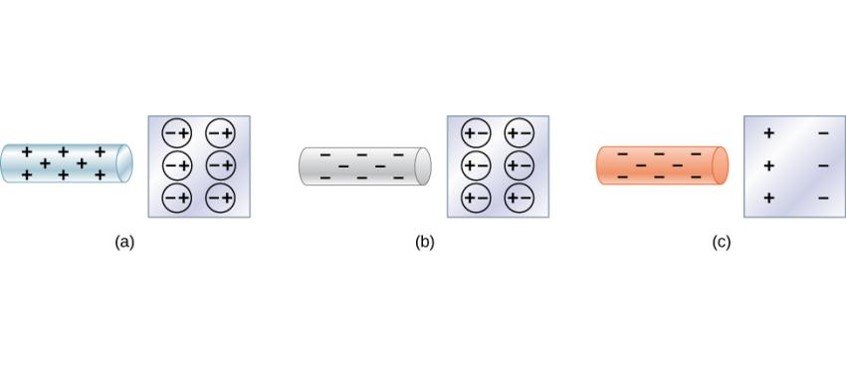
\includegraphics[scale=0.60]{fig/fig_05_11.jpg}
\caption{Attraction to neutral objects}
\label{fig:05_11}
\end{center}
\end{figure}

Charging by induction.
\begin{itemize}
\item Two uncharged or neutral metal spheres are in contact with each other but insulated from the rest of the world.
\item A positively charged glass rod is brought near the sphere on the left, attracting negative charge and leaving the other sphere positively charged.
\item The spheres are separated before the rod is removed, thus separating negative and positive charges.
\item The spheres retain net charges after the inducing rod is removed—without ever having been touched by a charged object.
\end{itemize}

\begin{figure}[h]
\begin{center}
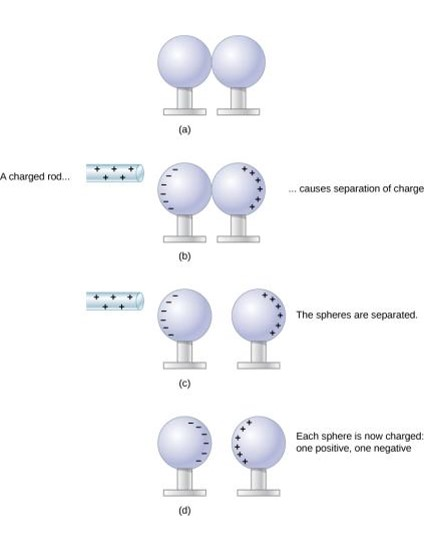
\includegraphics[scale=0.60]{fig/fig_05_12.jpg}
\caption{Charge by Induction}
\label{fig:05_12}
\end{center}
\end{figure}

Similarly using a ground connection

\begin{figure}[H]
\begin{center}
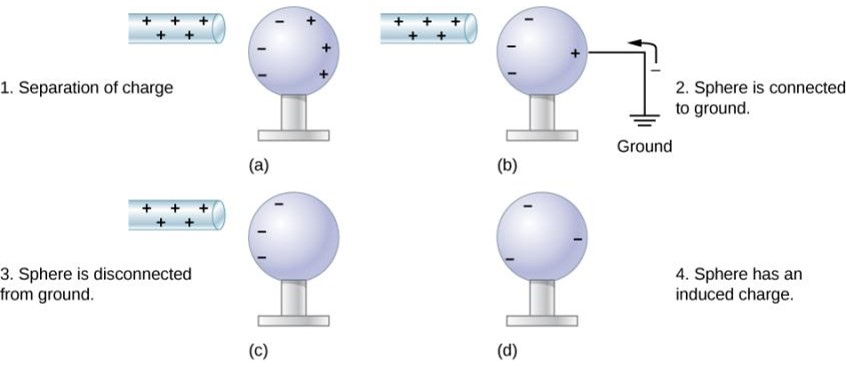
\includegraphics[scale=0.60]{fig/fig_05_13.jpg}
\caption{Charge by Induction with Ground Connection}
\label{fig:05_13}
\end{center}
\end{figure}

\section{Coulombs Law}

Recall from Physics I the gravitational force equation

\begin{figure}[h]
\begin{center}
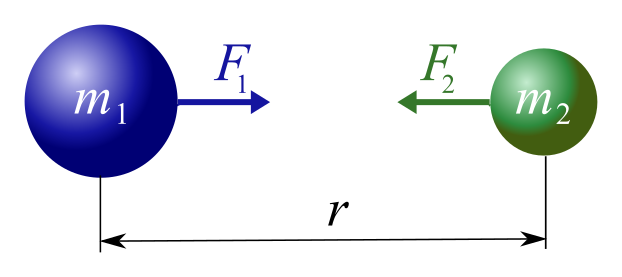
\includegraphics[scale=0.60]{fig/NewtonsLawGravitation.png}
\caption{Newtons Law Gravitation}
\label{fig:NLG}
\end{center}
\end{figure}

\begin{equation}
F_G = G \frac{m_1 m_2}{r^{2}}
\end{equation}



For the electric force, let
\begin{itemize}
\item $q_1, q_2 = $ the net electric charges of two objects
\item $\vec{r}_{12} = $ the vector displacement from $q_1$ to $q_2$.
\end{itemize}

\begin{equation}
F \propto \frac{q_1 q_2}{r^{2}_{12}}
\end{equation}

\begin{figure}[h]
\begin{center}
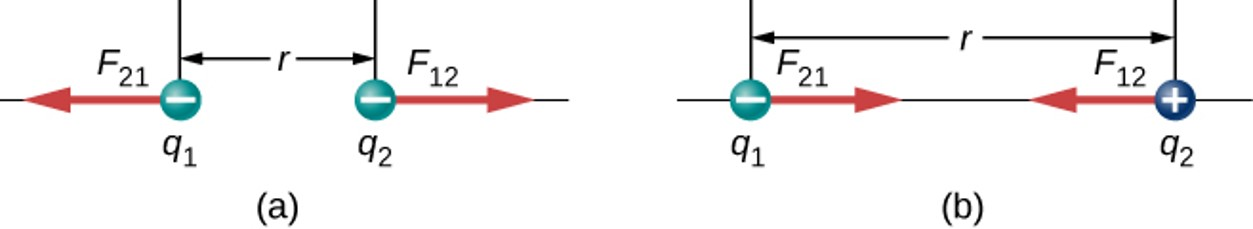
\includegraphics[scale=0.60]{fig/fig_05_14.jpg}
\caption{Electrostatic Force}
\label{fig:05_14}
\end{center}
\end{figure}

Coulomb's Law: the electric force between two electrically charged particles is given by

\begin{equation}
\vec{F} = \frac{1}{4 \pi \epsilon_0} \frac{q_1 q_2}{r^{2}_{12}} \hat{r}_{12}
\end{equation}

where $\vec{r}_{12}$ is the unit vector from particle 1 to particle 2, and 
where $\epsilon_0$ is the permittivity of free space

\begin{equation}
\epsilon_0 = 8.85 * 10^{-12} \frac{C^2}{N \cdot m^2}
\end{equation}

Which leads to Coulomb's constant ($k$):

\begin{equation}
k_e = \frac{1}{4 \pi \epsilon_0} = 8.99 * 10^9 \frac{N \cdot m^2}{C^2} 
\end{equation}


\subsection{Example: Force on the Electron in a Hydrogen Atom}

Proton has a positive charge of $+e$, and an electron has a negative charge of $-e$. In the "ground state" of the atom, the electron orbits the proton at a probably distance of $5.29 * 10^{-11} m$.

\begin{equation}
q_1 = +e = +1.602 * 10^{-19} C 
\end{equation}

\begin{equation}
q_2 = -e = -1.602 * 10^{-19} C 
\end{equation}

\begin{equation}
r = 5.29 * 10^{-11} m
\end{equation}

The magnitude of the force

\begin{equation}
F = \frac{1}{4 \pi \epsilon_0} \frac{\lvert e \lvert^2}{r^{2}} = 8.99 * 10^9 \frac{N \cdot m^2}{C^2} * \frac{(1.602 * 10^{-19} C)^2}{(5.29 * 10^{-11} m)^2} = 8.25 * 10^{-8} N
\end{equation}

The force is thus expressed as

\begin{equation}
\vec{F} = (8.25 * 10^{-8} N) \hat{r}
\end{equation}

\subsection{Multiple Sources of Charge}

As with the forces encountered in Physics I, the net electric force is the vector sum of the individual forces. 

\begin{equation}
\vec{F}(r) = \frac{1}{4 \pi \epsilon_0} Q \sum_{i=1}^{N}\frac{q_i}{r_i^2}\hat{r}_i
\end{equation}

where $Q$ represents the charge of a particle that experiences the force $\vec{F}$ and is located at $\vec{r}$ from the origin; $q_i$ are the N source charges, and the vectors $\vec{r}_i = r_i \hat{r}_i$ are the displacements from the position of the ith charge to the position of Q. All of this is with the simplifying assumption that the source charges are all fixed in place somehow. This is referred to as the electrostatic force. 

\begin{figure}[h]
\begin{center}
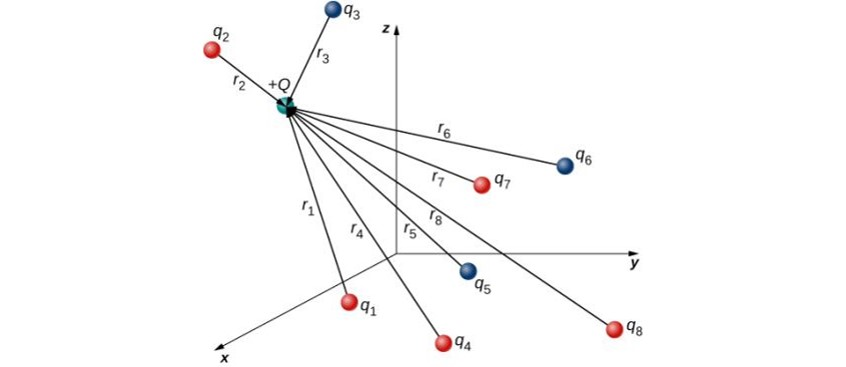
\includegraphics[scale=0.60]{fig/fig_05_15.jpg}
\caption{Multiple Source Charges}
\label{fig:05_15}
\end{center}
\end{figure}


insert example 5.2

\section{Electric Field}

Next we define the Electric Field, which is independent of the test charge Q, and only depends on the configuration of the source charges. 

\begin{equation}
\vec{F} = Q \cdot \vec{E}
\end{equation}

where 

\begin{equation}
\vec{E}(P) = \frac{1}{4 \pi \epsilon_0} \sum_{i=1}^{N}\frac{q_i}{r_i^2}\hat{r}_i
\end{equation}

expresses the Electric Field at position $P = P(x,y,z)$ of the N source charges. 

\begin{figure}[h]
\begin{center}
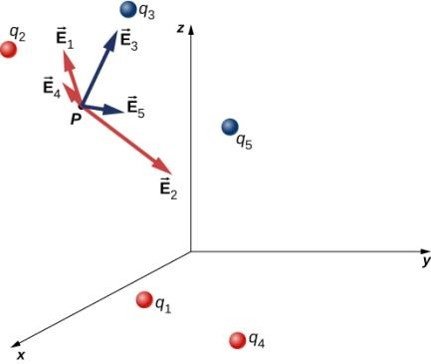
\includegraphics[scale=0.60]{fig/fig_05_18.jpg}
\caption{Electric Field - Multiple Source Charges}
\label{fig:05_18}
\end{center}
\end{figure}


This is analogous to the graviational field $\vec{g}$ of the Earth

\begin{equation}
\vec{g} = G \frac{M}{r^2}\hat{r}
\end{equation}

which gives us $9.81 \frac{m}{s}$ near the Earth's surface.


The Electric Field is
\begin{itemize}
\item A vector field
\item Obeys superposition
\item By convention, the Electric Field points away from the positive charge. 
\end{itemize}

\section{Calculating Electric Field Charge Distributions}

\begin{figure}[h]
\begin{center}
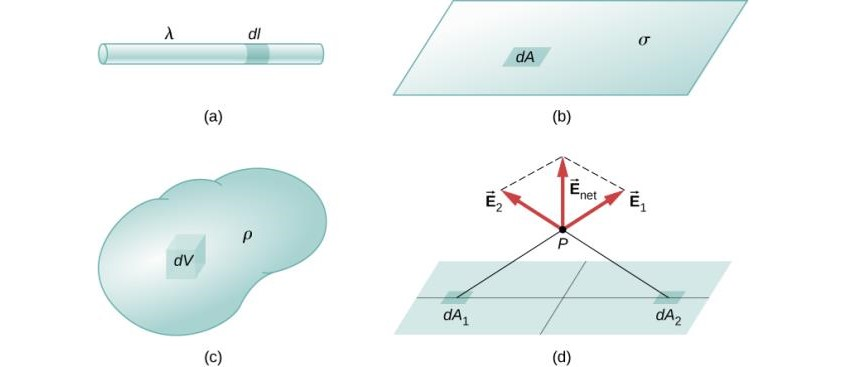
\includegraphics[scale=0.60]{fig/fig_05_22.jpg}
\caption{Configuration of Charge}
\label{fig:05_22}
\end{center}
\end{figure}

Definitions of charge density
\begin{itemize}
\item $\lambda \equiv $ charge per unit length (linear charge density) in $\frac{C}{m}$
\item $\sigma \equiv $ charge per unit area (surface charge density) in $\frac{C}{m^2}$
\item $\rho \equiv $ charge per unit volume (volume charge density) in $\frac{C}{m^3}$
\end{itemize}

Given these densities, the differential charge ($dq$) becomes $\lambda dl$, $\sigma dA$, and $\rho dV$, respectively. 

For these distributions, the summation becomes an integral
\begin{itemize}
\item Point Charge
	\begin{equation}
	\vec{E}(P) = \frac{1}{4 \pi \epsilon_0} \sum_{i=1}^{N}\frac{q_i}{r^2}\hat{r}
	\end{equation}
\item Line Charge
	\begin{equation}
	\vec{E}(P) = \frac{1}{4 \pi \epsilon_0} \int_{line}(\frac{\lambda dl}{r^2})\hat{r}
	\end{equation}
\item Surface Charge
	\begin{equation}
	\vec{E}(P) = \frac{1}{4 \pi \epsilon_0} \int_{line}(\frac{\sigma dA}{r^2})\hat{r}
	\end{equation}
\item Surface Charge
	\begin{equation}
	\vec{E}(P) = \frac{1}{4 \pi \epsilon_0} \int_{line}(\frac{\rho dV}{r^2})\hat{r}
	\end{equation}
	
\end{itemize}

As $P = P(x,y,z)$:

\begin{equation}
\vec{E}_x(P) = \frac{1}{4 \pi \epsilon_0} \int_{line}(\frac{\lambda dl}{r^2})_x,
\vec{E}_y(P) = \frac{1}{4 \pi \epsilon_0} \int_{line}(\frac{\lambda dl}{r^2})_y,
\vec{E}_z(P) = \frac{1}{4 \pi \epsilon_0} \int_{line}(\frac{\lambda dl}{r^2})_z
\end{equation}


\subsection{Electric Field of a Line Segment}

\begin{figure}[h]
\begin{center}
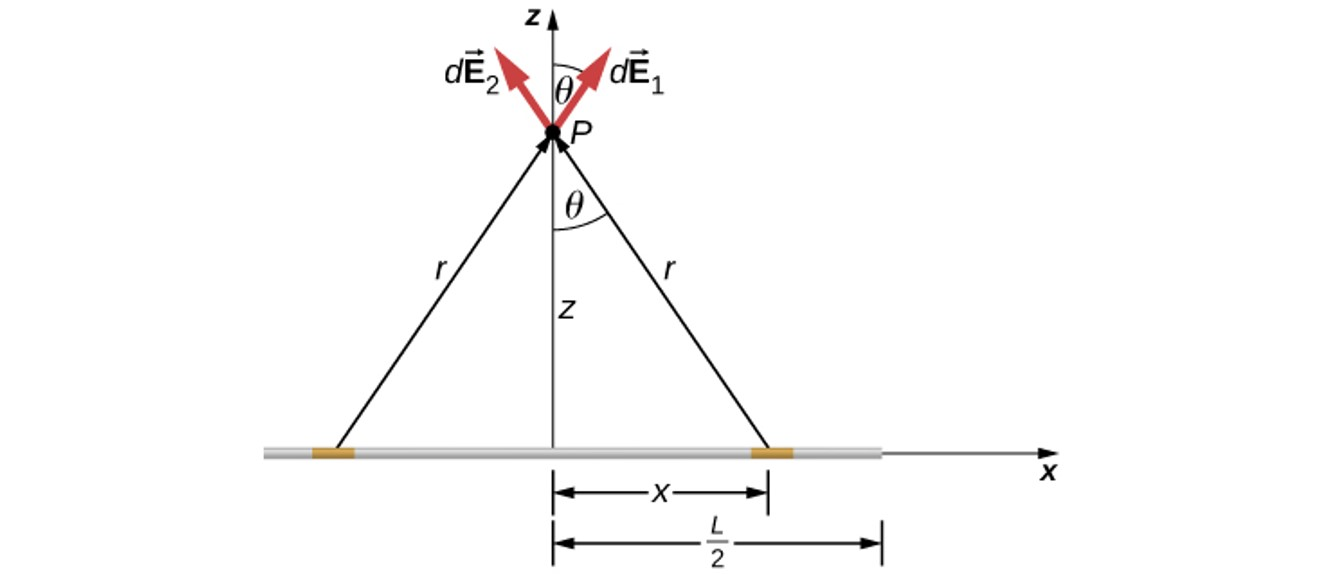
\includegraphics[scale=0.60]{fig/fig_05_23.jpg}
\caption{A uniformly charged segment of wire. The electric field at point P can be found by applying the superposition principle to symmetrically placed charge elements and integrating.
}
\label{fig:05_23}
\end{center}
\end{figure}


Start with 

\begin{equation}
\vec{E}(P) = \frac{1}{4 \pi \epsilon_0} \int_{line}(\frac{\lambda dl}{r^2})\hat{r}
\label{Eline}
\end{equation}
	
The symmetry of the arrangement implies the horizontal components cancel.

\begin{equation}
\vec{E}(P) = \vec{E^1} + \vec{E^2} = E_{1,x} \hat{i} + E_{1,z} \hat{k} + E_{2,x} (-\hat{i}) + E_{2,z} \hat{k}
\end{equation}

Due to symmetry, $E_{1,x} = E_{2,x}$, and as their directions are opposite, they cancel. So,

\begin{equation}
\vec{E}(P) = E_{1,z} \hat{k}  + E_{2,z} \hat{k} = E_1 \cos{\theta} \hat{k} + E_2 \cos{\theta} \hat{k}
\end{equation}

As these components are also equal, substituting into Equation \ref{Eline} yields:

\begin{equation}
\vec{E}(P) = \frac{1}{4 \pi \epsilon_0} \int_{0}^{\frac{L}{2}}(\frac{2 \lambda dx}{r^2} \cos{\theta})\hat{k}
\end{equation}

To calculate the integral, we note that 

\begin{equation}
r = \sqrt{(x^2 + z ^2)}
\end{equation}

and

\begin{equation}
\cos{\theta} = \frac{z}{r} = \frac{z}{\sqrt{(x^2 + z ^2)}} =  \frac{z}{(x^2 + z ^2)^{\frac{1}{2}}}
\end{equation}

Substituting

\begin{equation}
\vec{E}(P) = \frac{1}{4 \pi \epsilon_0} \int_{0}^{\frac{L}{2}}(\frac{2 \lambda dx}{(x^2 + z ^2)} \frac{z}{(x^2 + z ^2)^{\frac{1}{2}}})\hat{k}
\end{equation}

\begin{equation}
\vec{E}(P) = \frac{1}{4 \pi \epsilon_0} \int_{0}^{\frac{L}{2}}(\frac{2 \lambda z}{(x^2 + z ^2)^{\frac{3}{2}}}) dx \hat{k}
\end{equation}

Integrating
\begin{equation}
\vec{E}(P) = \frac{2 \lambda z}{4 \pi \epsilon_0} [\frac{x}{z^2 \sqrt{(x^2 + z ^2)}}]\bigg\rvert_{0}^{\frac{L}{2}} \hat{k}
\end{equation}

or

\begin{equation}
\vec{E}(z) = \frac{1}{4 \pi \epsilon_0} \frac{\lambda L}{z \sqrt{(\frac{L}{4} + z^2)}} \hat{k}
\end{equation}

For an infinite line: $L = \infty$

\begin{equation}
\vec{E}(z) = \frac{1}{4 \pi \epsilon_0} \frac{2 \lambda}{z} \hat{k}
\end{equation}

noting that we lost the $\frac{1}{r^2}$ dependence

For a finite line of charge with $z >> L$

\begin{equation}
\vec{E}(z) = \frac{1}{4 \pi \epsilon_0} \frac{\lambda L}{z^2} \hat{k}
\end{equation}

Recalling that $q = \lambda L$, then we get the expression of the field of a point charge.



\section{Electric Field Lines}

Electric Field Lines allow us to visualize the electric field in space

\begin{figure}[H]
\begin{center}
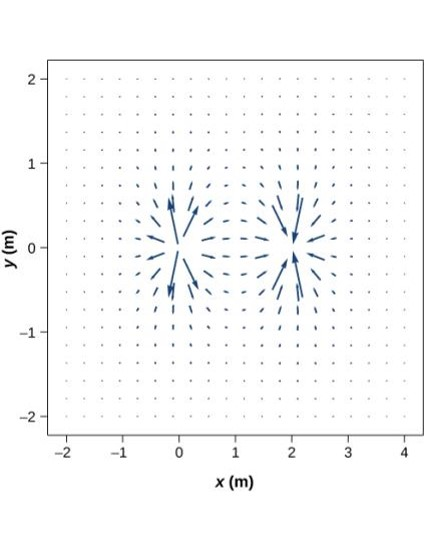
\includegraphics[scale=0.60]{fig/fig_05_28.jpg}
\caption{Vector field of dipole}
\label{fig:05_28}
\end{center}
\end{figure}

Electric Field Line "Rules"

\begin{itemize}
\item Either begin at a positive charge or come in from infinity
\item Either end at a negative charge or extend out to infinity
\item The number of lines originating or terminating is proportional to the amount of charge.
\item The density at any point in space is proportional to (and therefore is representative of) the magnitude of the field at that point in space 
\item The field lines never cross
\end{itemize}

\begin{figure}[h]
\begin{center}
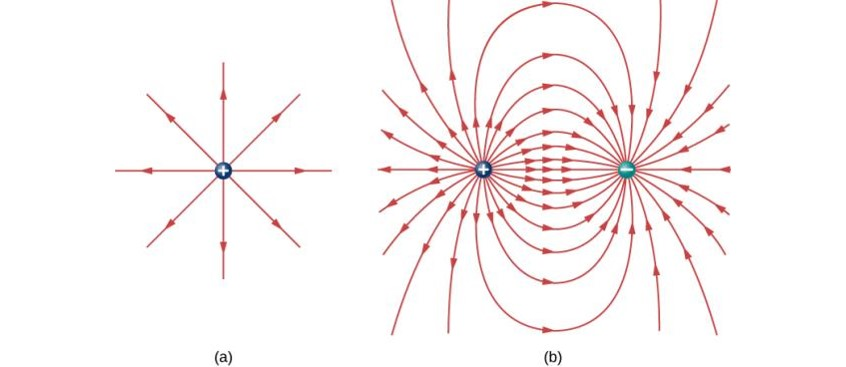
\includegraphics[scale=0.60]{fig/fig_05_29.jpg}
\caption{Electric Field of a dipole}
\label{fig:05_29}
\end{center}
\end{figure}

\begin{figure}[h]
\begin{center}
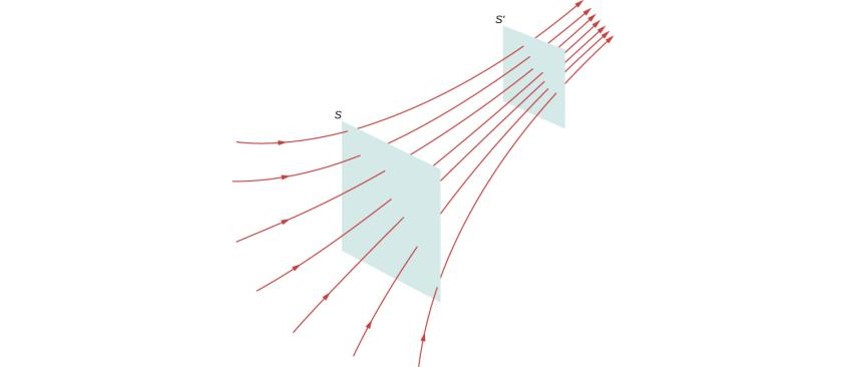
\includegraphics[scale=0.60]{fig/fig_05_30.jpg}
\caption{Field Line Density}
\label{fig:05_30}
\end{center}
\end{figure}

\begin{figure}[h]
\begin{center}
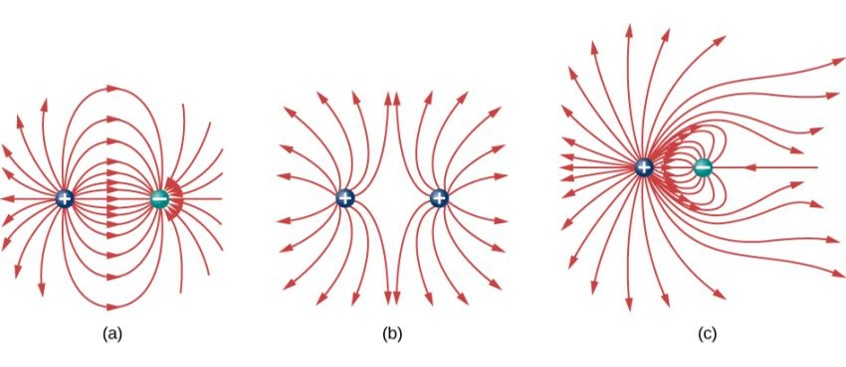
\includegraphics[scale=0.60]{fig/fig_05_31.jpg}
\caption{Typical Diagrams}
\label{fig:05_31}
\end{center}
\end{figure}

\chapter{Module 2: Chapter 6 - Gauss's Law}

Four main topics:

\begin{itemize}
\item Electric Flux
\item Guass's Law
\item Calculating Electric Field with Guass's Law
\item Electric Field inside Conductors
\end{itemize}


\section{Electric Flux}

Flux describes how much of something goes through a given area. More formally, flux is the dot-product of a vector field (in our case, the electric field) with an area.  

\begin{figure}[h]
\begin{center}
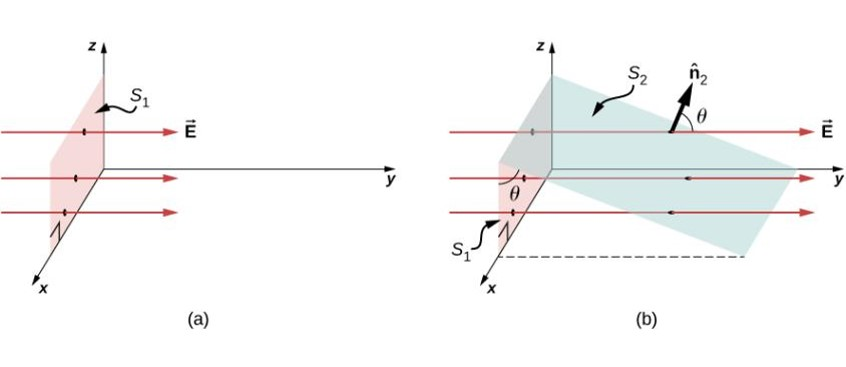
\includegraphics[scale=0.60]{fig/fig_06_04.jpg}
\caption{Flux through a plane}
\label{fig:06_04}
\end{center}
\end{figure}

\subsection{Electric Flux}

For uniform field $\vec{E}$ and a flat surface:
\begin{equation}
\Phi = \vec{E} \cdot \vec{A}
\end{equation}
\begin{equation}
\Phi = E A \cos{\theta}
\end{equation}


\begin{figure}[H]
\begin{center}
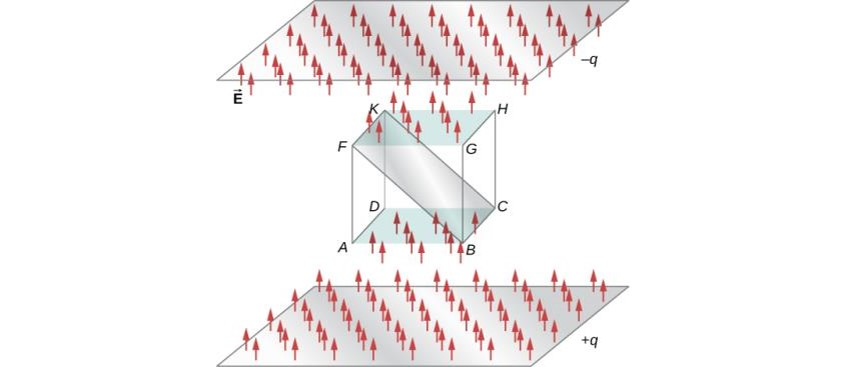
\includegraphics[scale=0.60]{fig/fig_06_07.jpg}
\caption{Flux through a cube}
\label{fig:06_07}
\end{center}
\end{figure}

\begin{itemize}
\item Source and termination of electric field lines are outside the cube
\item There is no charge inside the cube
\item All electric field lines that enter the cube exit it, so the net flux through the cube is zero.
\item By convention: if field lines are leaving a closed surface then $\Phi$ is positive. 
\item For field lines entering a closed surface, $\Phi$ is negative.
\end{itemize}

For a non-flat surface, we can take small patches that approximate a flat surface

\begin{figure}[H]
\begin{center}
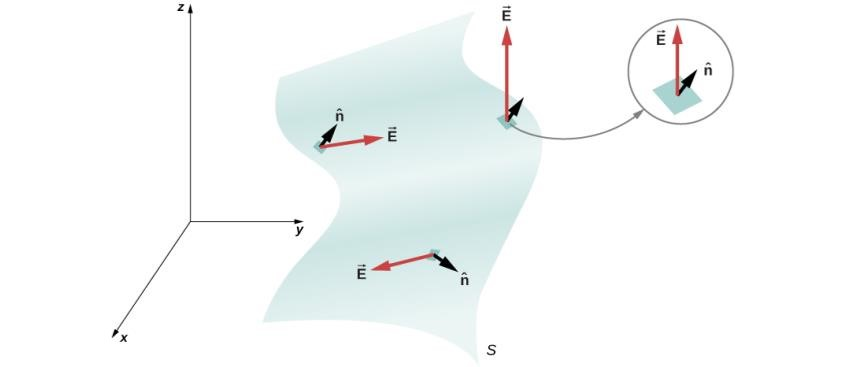
\includegraphics[scale=0.60]{fig/fig_06_08.jpg}
\caption{Surface divided into patches to find flux}
\label{fig:06_08}
\end{center}
\end{figure}

Consider $\vec{E}_i$ to be the electric field over the $i^{th}$ patch ($\delta A_i$, then

\begin{equation}
\Phi_i = \vec{E}_i \cdot \delta \vec{A}_i
\end{equation}

then

\begin{equation}
\Phi = \sum_{i=1}^{N} \Phi_i = \sum_{i=1}^{N} \vec{E}_i \cdot \delta \vec{A}_i
\end{equation}

As the patch gets infinitesimally small, 

\begin{equation}
\delta \vec{A} \rightarrow \hat{n} dA
\end{equation}

and the $\sum$ become an $\int_s$ over the entire surface

For an Open Surface:

\begin{equation}
\Phi = \int_s \vec{E} \cdot \hat{n} dA = \int_s \vec{E}  \cdot d\vec{A}
\end{equation}

For an Closed Surface:

\begin{equation}
\Phi = \oint_s \vec{E} \cdot \hat{n} dA = \oint_s \vec{E}  \cdot d\vec{A}
\label{eq:flux}
\end{equation}

\section{Gauss's Law}

Let's calculate the electric flux through a sphere that surrounds a point charge $q$.

Recall at Point $P$
\begin{equation}
\vec{E}_P = \frac{1}{4 \pi \epsilon_0} \frac{q}{r^2} \hat{r}
\end{equation}

where $\hat{r}$ is the radial unit vector charge at the center to Point $P$.

\begin{figure}[H]
\begin{center}
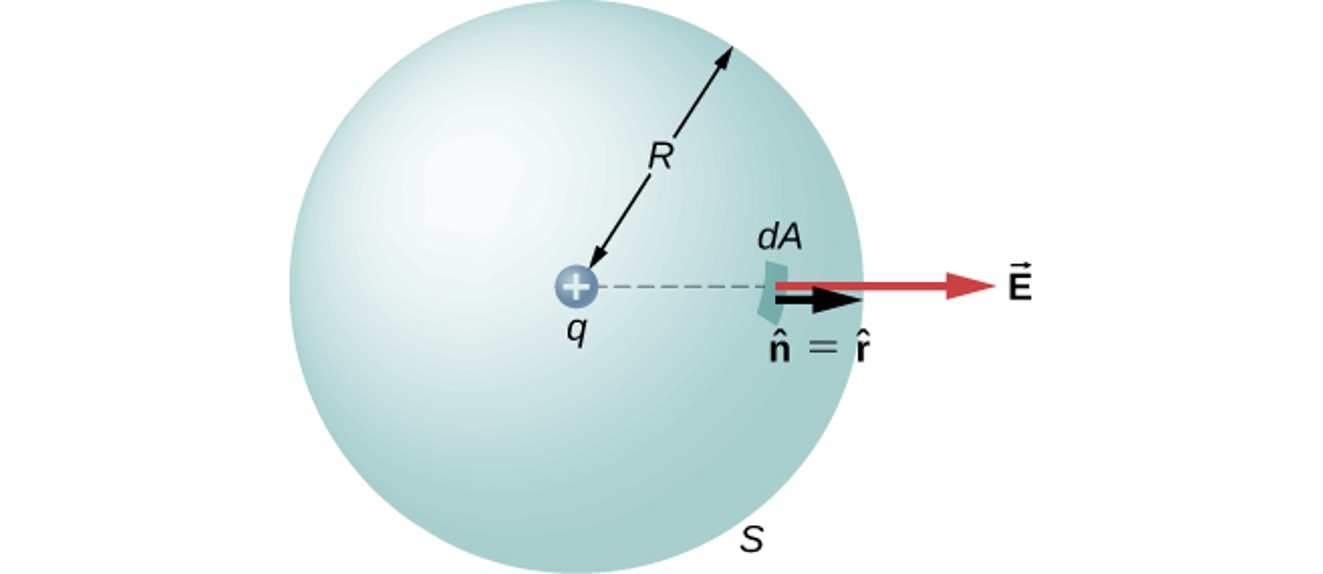
\includegraphics[scale=0.40]{fig/fig_06_13.jpg}
\caption{Closed sphere around point charge P}
\label{fig:06_13}
\end{center}
\end{figure}

Applying the flux equation \ref{eq:flux}, where $\hat{n} = \hat{r}$ and $r = R$, for infinitesimal area $dA$:

\begin{equation}
d\Phi = \vec{E} \cdot \hat{n} dA = \frac{1}{4 \pi \epsilon_0} \frac{q}{R^2} \hat{r} \cdot \hat{r} dA =  \frac{1}{4 \pi \epsilon_0} \frac{q}{R^2} dA
\end{equation}

Integrating

\begin{equation}
\Phi = \frac{1}{4 \pi \epsilon_0} \frac{q}{R^2} \oint_s dA =  \frac{1}{4 \pi \epsilon_0} \frac{q}{R^2} (4 \pi R^2) = \frac{q}{\epsilon_0}
\end{equation}

As r increases, there is a  $\frac{1}{r^2}$ decrease in electric field counteracts the $r^2$ increase in the surface of the sphere and we find that $\Phi = \frac{q}{\epsilon_0}$ is independent of the size of the sphere. 


Gauss's Law
\begin{equation}
\boxed{\Phi_{closedsurface} = \frac{q_{enc}}{\epsilon_0}}
\end{equation}

where $q_{enc}$ is the net charge enclosed by the surface

\section{Applying Gauss's Law}

\subsubsection{Charge Distribution with Spherical Symmetry}

Charge distribution is considered spherically symmetric if the density of charge depends only on the distance from a point in space and not direction. A spherically symmetric charge distribution does not change of you rotate the sphere.

\begin{equation}
\rho(r,\theta,\phi) = \rho(r)
\end{equation}

For spherically symmetric:

\begin{equation}
\vec{E}_P = E_P(r)\hat{r}
\end{equation}

The magnitude of the electric field $\vec{E}$ is the same everywhere on a spherical Gaussian surface concentric with the distribution. For a sphere of radius $r$:

\begin{equation}
\Phi = E_P 4 \pi r^2
\end{equation}

From Gauss's Law
\begin{equation}
4 \pi r^2 E = \frac{q_{enc}}{\epsilon_0}
\end{equation}

Combining, the magnitude $E(r)$ is given by
\begin{equation}
E(r) = \frac{1}{4 \pi \epsilon_0}\frac{q_{enc}}{r^2}
\end{equation}

For a sphere of radius $R$

\begin{equation}
  q_{enc}=\begin{cases}
    q_{tot}, & \text{if } r \geq R.\\
    q_{(r<R)}, & \text{if } r < R.
  \end{cases}
\end{equation}

Which leads to an Electric Field at point P ($E_{out}$ for P outside the sphere, and $E_{in}$ for P inside the sphere

\begin{figure}[H]
\begin{center}
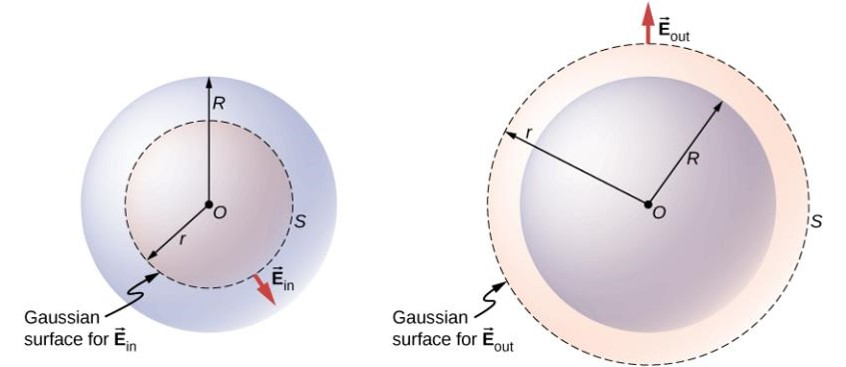
\includegraphics[scale=0.60]{fig/fig_06_23.jpg}
\caption{Outside and inside the sphere}
\label{fig:06_23}
\end{center}
\end{figure}

\begin{equation}
E_{out} = \frac{1}{4 \pi \epsilon_0}\frac{q_{tot}}{r^2}
\end{equation}

\begin{equation}
E_{in} = \frac{1}{4 \pi \epsilon_0}\frac{q_{(r<R)}}{r^2}
\end{equation}

So, what is $q_{enc}$ inside the sphere

\begin{equation}
q_{enc} = \int \rho_0 dV = \int_{0}^{r} \rho_0 4 \pi r^{\prime} dr^{\prime} = \rho_0 (\frac{4}{3} \pi r^3)
\end{equation}

Therefore

\begin{equation}
E_{out} = \frac{1}{4 \pi \epsilon_0}\frac{q_{tot}}{r^2}, \text{with} q_{tot} = \frac{4}{3} \pi R^3 \rho_0
\end{equation}

\begin{equation}
E_{in} = \frac{1}{4 \pi \epsilon_0}\frac{q_{(r<R)}}{r^2} = \frac{\rho_0 r}{3 \epsilon_0} \text{  since  } q_{(r<R)} = \frac{4}{3} \pi r^3 \rho_0
\end{equation}

\begin{figure}[H]
\begin{center}
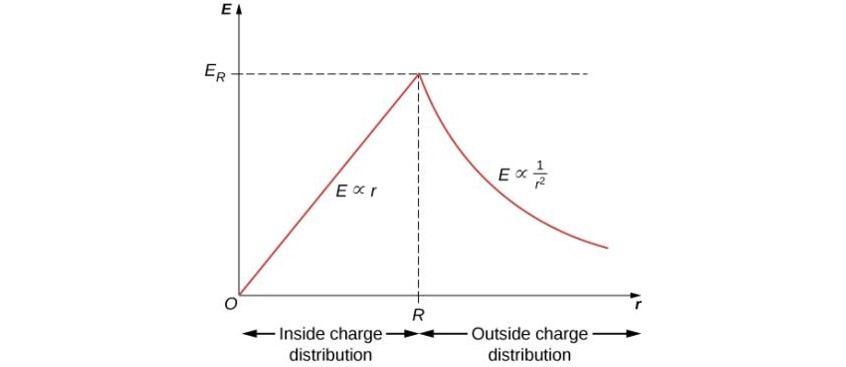
\includegraphics[scale=0.40]{fig/fig_06_24.jpg}
\caption{Electric Field of uniformly charged non-conducting sphere}
\label{fig:06_24}
\end{center}
\end{figure}

\subsubsection{Charge Distribution with Symmetric Cylinder}

Charge distribution is considered cylindrical symmetric if the density of charge depends only on the distance $r$ from the axis, and does not vary along or with direction of axis.

Consider an "infinitely\footnote{In the real world, cylinders are not finite, but if the length $L >> r$ then it can be approximated as infinitely long} cylinder with cylindrical symmetric charge distribution.

\begin{equation}
\rho(r,\theta,z) = \rho(r)
\end{equation}

\begin{equation}
\vec{E}_P = E_P(r)\hat{r}
\end{equation}


\begin{figure}[H]
\begin{center}
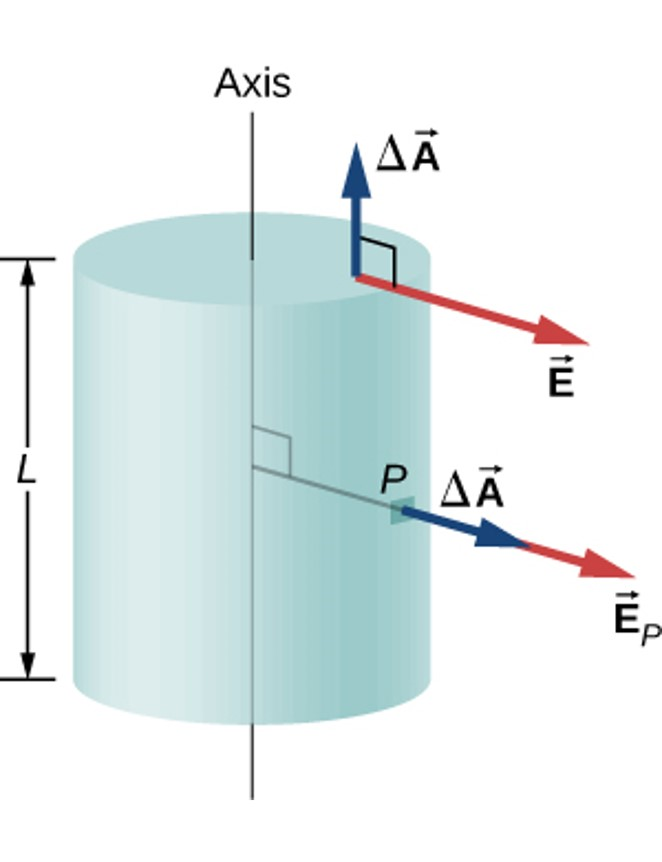
\includegraphics[scale=0.40]{fig/fig_06_29.jpg}
\caption{Cylindrically symmetric of length L}
\label{fig:06_29}
\end{center}
\end{figure}

The electric field is perpendicular to the sides and parallel to the end caps.

The flux through the cylinder part is

\begin{equation}
\int_s \vec{E} \cdot \hat{n} dA = E \int_s dA = E(2 \pi r L)
\end{equation}

and the flux through the caps is zero, because

\begin{equation}
\vec{E} \cdot \hat{n} = 0
\end{equation}

The total flux is then 

\begin{equation}
\int_s \vec{E} \cdot \hat{n} dA = 2 \pi r L E + 0 + 0 = 2 \pi r L E
\end{equation}

Using Gauss's law and taking $\lambda_{enc}$ to be the charge per unit length

\begin{equation}
q_{enc} = \lambda_{enc} L
\end{equation}

\begin{equation}
\Phi = 2 \pi r L E = \frac{q_{enc}}{\epsilon_0}
\end{equation}

The magnitude of $\vec{E}$
\begin{equation}
E(r)  = \frac{\lambda_{enc}}{2 \pi \epsilon_0} \frac{1}{r}
\end{equation}

\begin{equation}
  \lambda_{enc} L =\begin{cases}
    q_{tot}, & \text{if } r \geq R.\\
    q_{(r<R)}, & \text{if } r < R.
  \end{cases}
\end{equation}

What happens of it is a cylindrical shell vs a solid cylinder?

Consider surface charge density of $\sigma_0$.

\begin{figure}[H]
\begin{center}
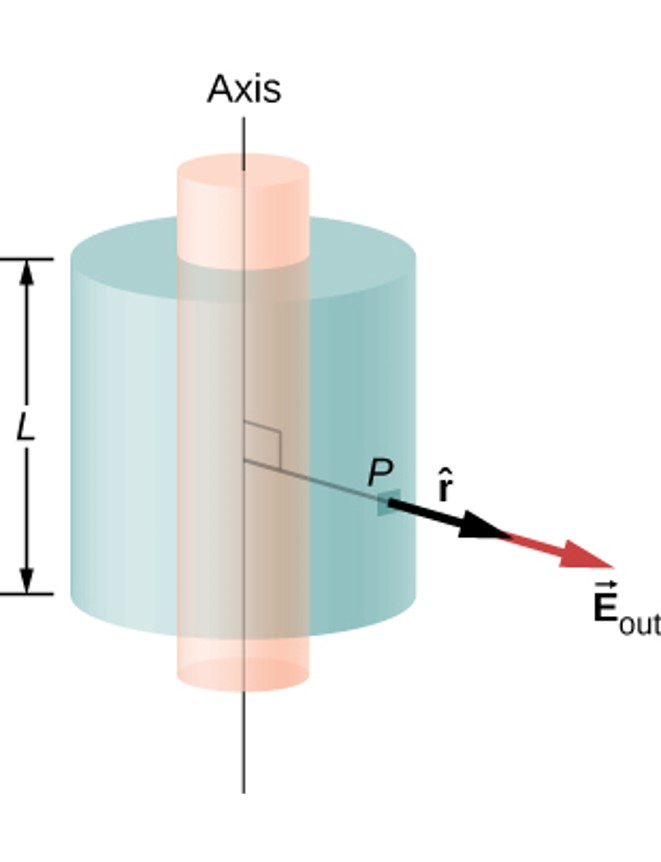
\includegraphics[scale=0.40]{fig/fig_06_30.jpg}
\caption{Guassian surface around a cylinderical shell}
\label{fig:06_30}
\end{center}
\end{figure}

\begin{equation}
\lambda_{enc} = \frac{\sigma_0 2 \pi R L}{L} = 2 \pi R \sigma_0
\end{equation} 

For point $P$ outside of the shell $r \geq R$:

\begin{equation}
\vec{E} = \frac{2 \pi R \sigma_0}{2 \pi \epsilon_0} \frac{1}{r} \hat{r}
\end{equation}

For point $P$ inside of the shell $r < R$:

\begin{equation}
\lambda_{enc} = 0
\end{equation}

so

\begin{equation}
\vec{E} = 0
\end{equation}

\section{Conductors in Electrostatic Equilibrium}
Moving from insulators to conductors. The electric field in conductors exerts a force on the free electrons (conduction electrons). As these electrons are not bound to an atom, they accelerate. However, moving charges are not static, so when electrostatic equilibrium is reached the charges are distributed in such a way that the electric field inside the conductor vanishes. 

\subsection{Electric Field inside a Conductor vanishes}

\begin{figure}[H]
\begin{center}
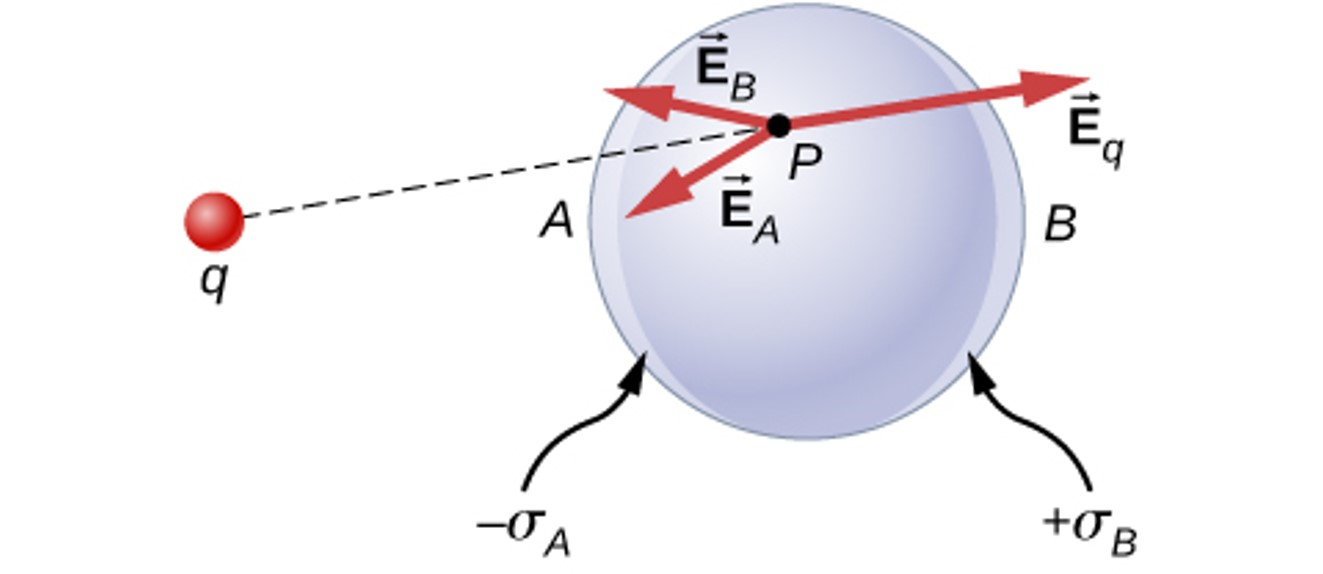
\includegraphics[scale=0.40]{fig/fig_06_35.jpg}
\caption{Metallic Sphere in presence of point charge}
\label{fig:06_35}
\end{center}
\end{figure}


The redistribution of charges is such that 
\begin{equation}
\vec{E}_P = \vec{E}_q + \vec{E}_A + \vec{E}_B = \vec{0}
\end{equation}

for induced charge $-\sigma_A$ and $+\sigma_B$

There is no net charge enclosed by a Gaussian surface that is solely within the volume of a conductor at equilibrium. This gives us $q_{enc} = 0$ and 

The redistribution of charges is such that 
\begin{equation}
\vec{E}_{net} = \vec{0} \text{   at points inside a conductor}
\end{equation}

\subsection{Charge on a conductor}

A consequence of a conductor in static equilibrium is that excess charge will end up on the outer surface of the conductor regardless of its origin.

\begin{figure}[H]
\begin{center}
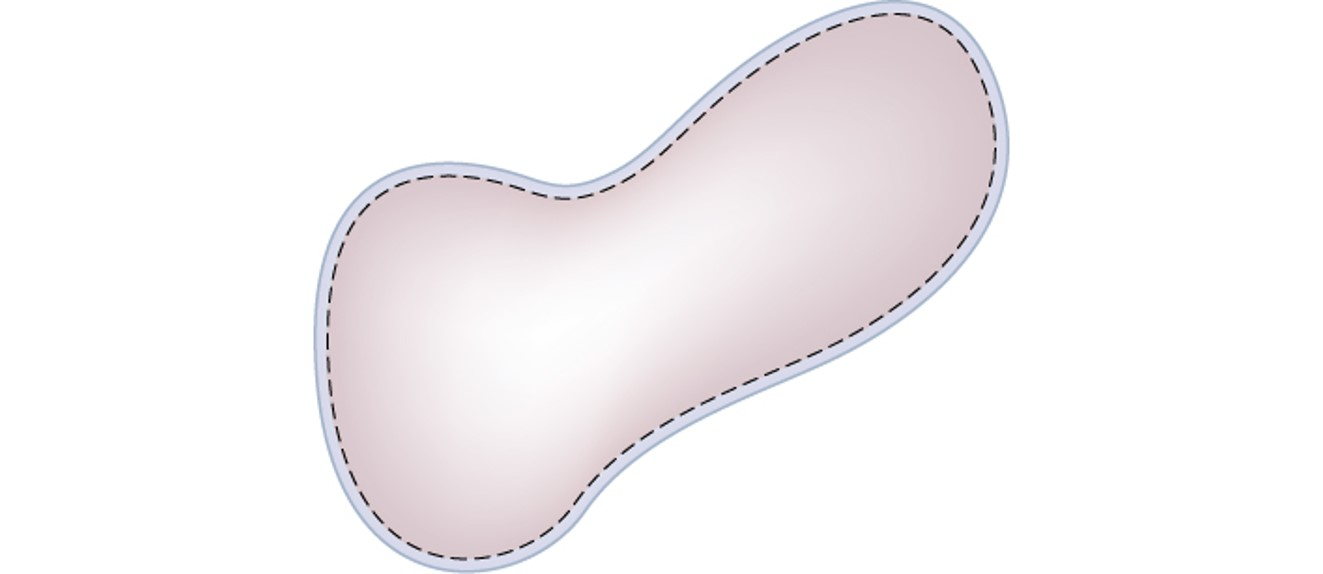
\includegraphics[scale=0.40]{fig/fig_06_37.jpg}
\caption{Gaussian surface just below conductor surface}
\label{fig:06_37}
\end{center}
\end{figure}

Since $E=0$ everywhere inside the conductor, 
\begin{equation}
\oint_s = \vec{E} \cdot \hat{n}dA = 0
\end{equation}

As the Gaussian surface lies infinitesimally below the actual surface, and there is no charge within the Gaussian surface, then all the excess charge must be on the surface. 

\subsection{Electric Field at the Surface of a Conductor}

If the electric field had a component parallel to the surface of the conductor, then the charges would move, which violates the electrostatic equilibrium assuming. Therefor the field must be normal to the surface. 

Just above the surface the magnitude of the electric field ($E$) and the surface charge density ($\sigma$) are related by

\begin{equation}
E = \frac{\sigma}{\epsilon_0}
\end{equation}

\begin{equation}
E = \frac{\sigma}{\epsilon_0}
\end{equation}

\begin{figure}[H]
\begin{center}
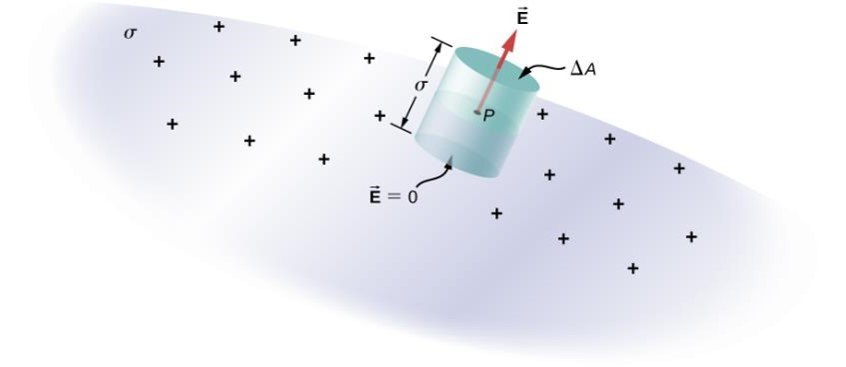
\includegraphics[scale=0.40]{fig/fig_06_39.jpg}
\caption{Field over the surface of a conductor}
\label{fig:06_39}
\end{center}
\end{figure}

Consider an infinitesimally small cylinder on the surface of a conductor with one face inside the conductor and one face outside. The height is $\delta$ and the cross section $\Delta A$. 

Given that $\Delta A$ is infinitesimally small, the total charge in the cylinder is $\sigma \Delta A$. 

The field is perpendicular to the surface, and thus the flux 
\begin{equation}
\Phi = E \Delta A = \frac{\sigma \Delta A}{\epsilon_0}
\end{equation}

yielding that charge right above the surface being given by:

\begin{equation}
E = \frac{\sigma}{\epsilon_0}
\end{equation}

\subsubsection{Electric Field of a Conducting Plate}

\begin{figure}[H]
\begin{center}
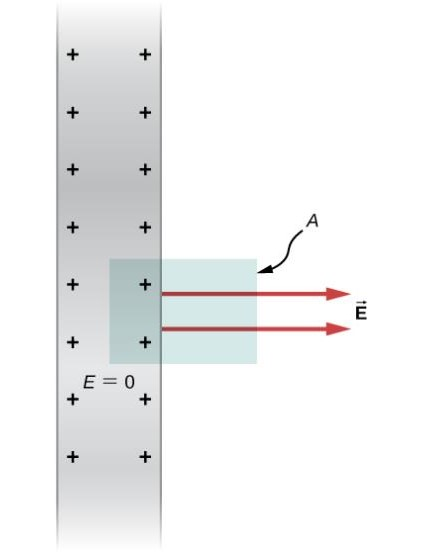
\includegraphics[scale=0.40]{fig/fig_06_40.jpg}
\caption{Conducting Plate}
\label{fig:06_40}
\end{center}
\end{figure}




\begin{figure}[H]
\begin{center}
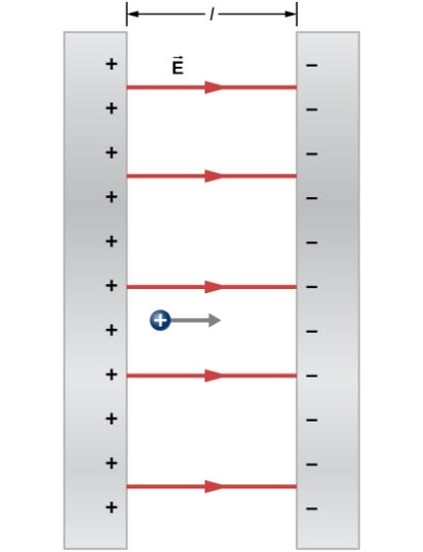
\includegraphics[scale=0.40]{fig/fig_06_41.jpg}
\caption{Between Conducting Plates}
\label{fig:06_41}
\end{center}
\end{figure}



\end{document}
